\documentclass[12pt]{report}
\usepackage[utf8]{inputenc}
\usepackage[russian]{babel}
%\usepackage[14pt]{extsizes}
\usepackage{listings}
\usepackage{graphicx}
\usepackage{amsmath,amsfonts,amssymb,amsthm,mathtools} 
\usepackage{pgfplots}
\usepackage{filecontents}
\usepackage{indentfirst}
\usepackage{eucal}
\usepackage{amsmath}
\usepackage{enumitem}
\frenchspacing

\usepackage{indentfirst} % Красная строка


%\usetikzlibrary{datavisualization}
%\usetikzlibrary{datavisualization.formats.functions}

\usepackage{amsmath}




% Для листинга кода:
\lstset{ %
language=haskell,                 % выбор языка для подсветки (здесь это С)
basicstyle=\small\sffamily, % размер и начертание шрифта для подсветки кода
numbers=left,               % где поставить нумерацию строк (слева\справа)
numberstyle=\tiny,           % размер шрифта для номеров строк
stepnumber=1,                   % размер шага между двумя номерами строк
numbersep=5pt,                % как далеко отстоят номера строк от подсвечиваемого кода
showspaces=false,            % показывать или нет пробелы специальными отступами
showstringspaces=false,      % показывать или нет пробелы в строках
showtabs=false,             % показывать или нет табуляцию в строках
frame=single,              % рисовать рамку вокруг кода
tabsize=2,                 % размер табуляции по умолчанию равен 2 пробелам
captionpos=t,              % позиция заголовка вверху [t] или внизу [b] 
breaklines=true,           % автоматически переносить строки (да\нет)
breakatwhitespace=false, % переносить строки только если есть пробел
escapeinside={\#*}{*)}   % если нужно добавить комментарии в коде
}

\usepackage[left=2cm,right=2cm, top=2cm,bottom=2cm,bindingoffset=0cm]{geometry}
% Для измененных титулов глав:
\usepackage{titlesec, blindtext, color} % подключаем нужные пакеты
\definecolor{gray75}{gray}{0.75} % определяем цвет
\newcommand{\hsp}{\hspace{20pt}} % длина линии в 20pt
% titleformat определяет стиль
\titleformat{\chapter}[hang]{\Huge\bfseries}{\thechapter\hsp\textcolor{gray75}{|}\hsp}{0pt}{\Huge\bfseries}


% plot
\usepackage{pgfplots}
\usepackage{filecontents}
\usetikzlibrary{datavisualization}
\usetikzlibrary{datavisualization.formats.functions}

\begin{document}
%\def\chaptername{} % убирает "Глава"
\thispagestyle{empty}
\begin{titlepage}
	\noindent \begin{minipage}{0.15\textwidth}
	
\includegraphics[width=\linewidth]{b_logo}
	\end{minipage}
	\noindent\begin{minipage}{0.9\textwidth}\centering
		\textbf{Министерство науки и высшего образования Российской Федерации}\\
		\textbf{Федеральное государственное бюджетное образовательное учреждение высшего образования}\\
		\textbf{~~~«Московский государственный технический университет имени Н.Э.~Баумана}\\
		\textbf{(национальный исследовательский университет)»}\\
		\textbf{(МГТУ им. Н.Э.~Баумана)}
	\end{minipage}
	
	\noindent\rule{18cm}{3pt}
	\newline\newline
	\noindent ФАКУЛЬТЕТ $\underline{\text{«Информатика и системы управления»}}$ \newline\newline
	\noindent КАФЕДРА $\underline{\text{«Программное обеспечение ЭВМ и информационные технологии»}}$\newline\newline\newline\newline\newline
	
	
	\begin{center}
		\noindent\begin{minipage}{1.3\textwidth}\centering
			\Large\textbf{  Домашнее задание по }\newline
			\textbf{ дисциплине <<Анализ алгоритмов>>}\newline\newline
		\end{minipage}
	\end{center}
	
	\noindent\textbf{Тема} $\underline{\text{Графовые модели программ}}$\newline\newline
	\noindent\textbf{Студент} $\underline{\text{Романов А.В.}}$\newline\newline
	\noindent\textbf{Группа} $\underline{\text{ИУ7-53Б}}$\newline\newline
	\noindent\textbf{Преподаватели} $\underline{\text{Волкова Л.Л., Строганов Ю.В.}}$\newline\newline\newline
	
	\begin{center}
		\vfill
		Москва~---~\the\year
		~г.
	\end{center}
\end{titlepage}


\tableofcontents

\newpage
\chapter{Исходный код алгоритма}

\begin{lstlisting}[label=some-code,caption=Функция умножения матриц по Винограду, language=C]
for (int i = 0; i < N1; ++i) {															(1)
	for (int j = 0; j < M1 / 2; ++j) {												(2)
		rows[i] += matrix1[i][j * 2] * matrix[i][j * 2 + 1]; 		(3)
	}
}

for (int i = 0; i < M2; ++i) {															(4)
	for (int j = 0; j < N2 / 2; ++j) {												(5)
		cols[i] += matrix1[j * 2][i] * matrix[j * 2 + 1][i];		(6)
	}
}

for (int i = 0; i < N1; ++i) {															(7)
	for (int j = 0; j < M2; ++j) {														(8)
		res[i][j] = -rows[i] - col[j];											  	(9)
		for (int k = 0; k < M1 / 2; ++k) {											(10)
			res[i][j] += (matrix1[i][2 * k + 1] +
			 			  matrix2[2 * k][j]) * (matrix1[i][2 * k] +
			  			matrix2[2 * k + 1][j]);												(11)
		}
	}
}

if (M1 % 2) {																								(12)
	for (int i = 0; i < N1; ++i) {														(13)
		for (int j = 0; j < M2; ++j) {													(14)
			res[i][j] += matrix1[i][M1 - 1] * matrix2[M1 - 1][j];	(15)
		}
	}
}
\end{lstlisting}

\chapter{Модели программ}

\section{Граф управления программы}

\begin{figure}[h]
	\centering
	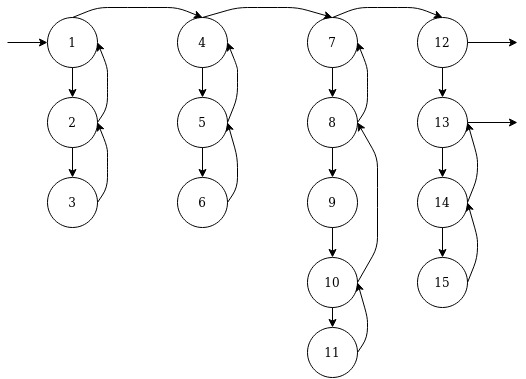
\includegraphics[scale=1]{control_graph.jpg}
	\caption{Граф управления программы}
	\label{fig:mpr}
\end{figure}

\section{Информационный граф программы}

\begin{figure}[h]
	\centering
	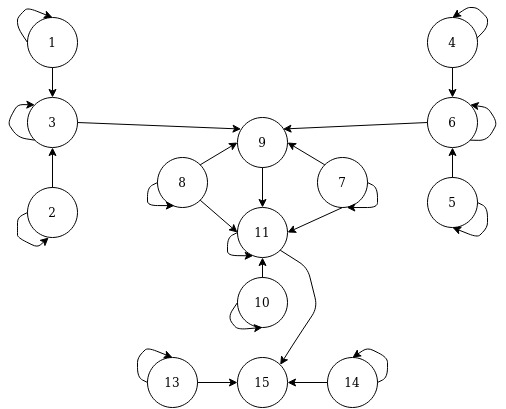
\includegraphics[scale=1]{info_graph.jpg}
	\caption{Информационный граф программы}
	\label{fig:mpr}
\end{figure}

\section{Операционная история программы}

\begin{figure}[h]
	\centering
	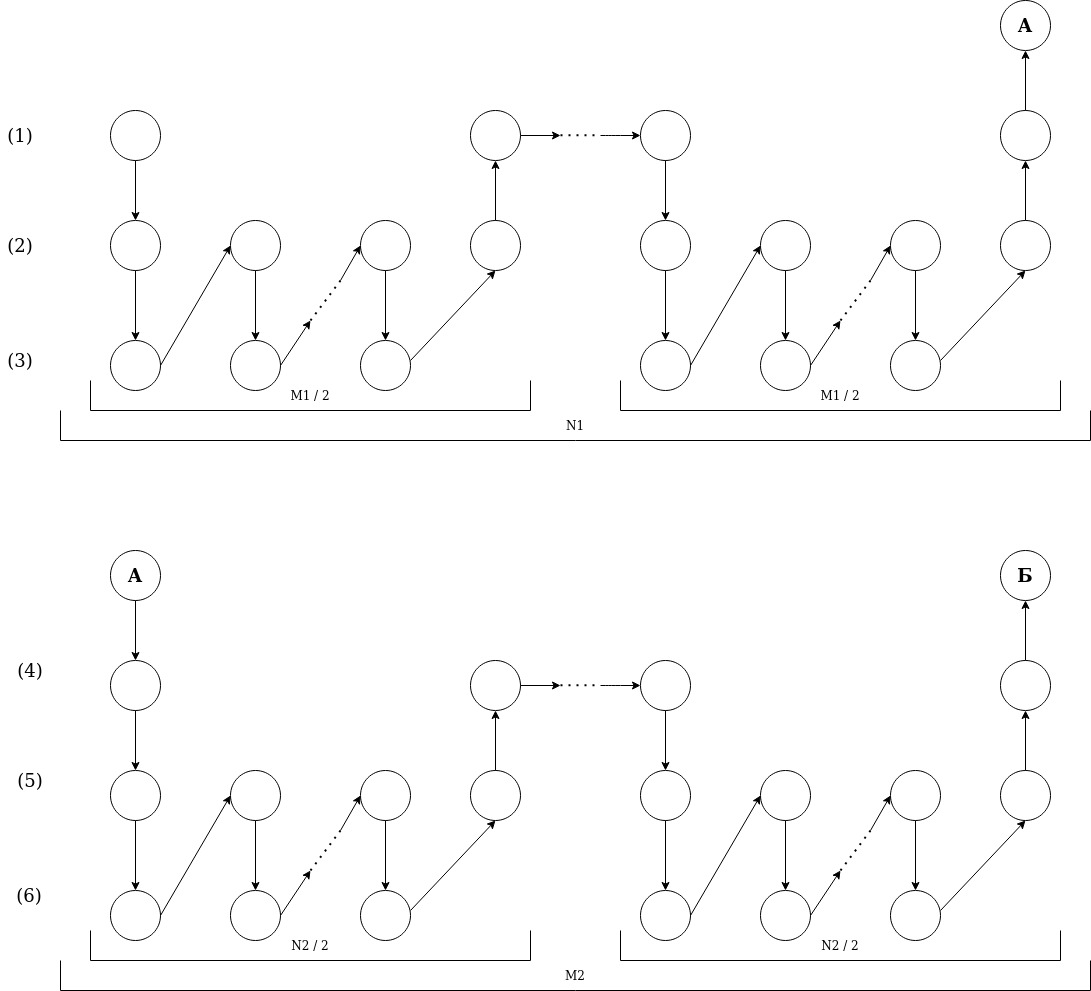
\includegraphics[scale=0.46]{oper_history_1.jpg}
	\caption{Операционная история программы, часть 1}
	\label{fig:mpr}
\end{figure}

\begin{figure}[h]
	\centering
	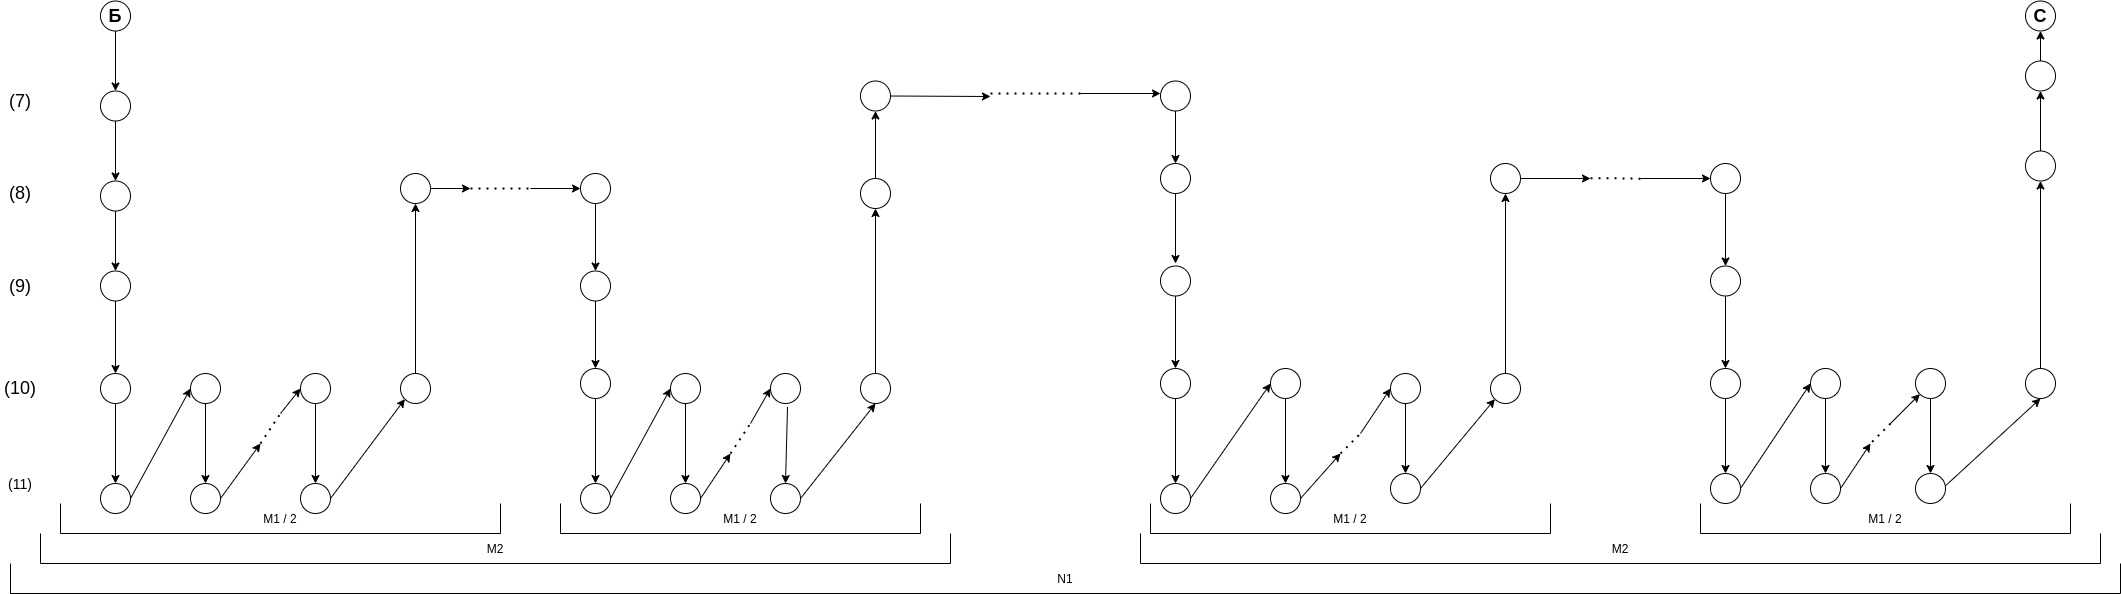
\includegraphics[scale=0.25]{oper_history_2.jpg}
	\caption{Операционная история программы, часть 2}
	\label{fig:mpr}
\end{figure}

\begin{figure}[h]
	\centering
	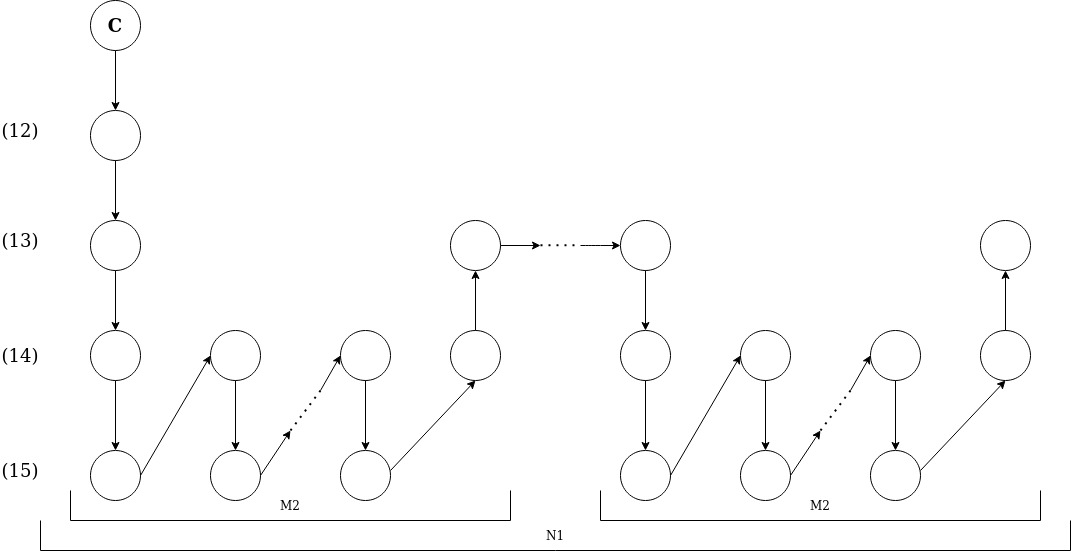
\includegraphics[scale=0.48]{oper_history_3.jpg}
	\caption{Операционная история программы, часть 3}
	\label{fig:mpr}
\end{figure}

\section{Информационная история программы}

\begin{figure}[h]
	\centering
	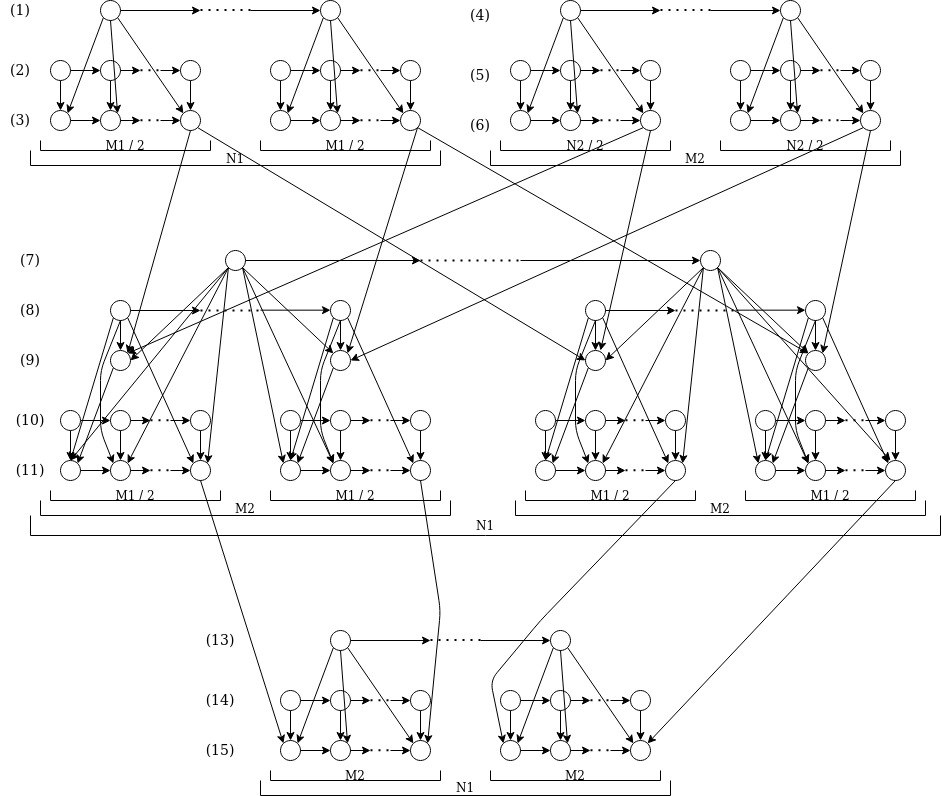
\includegraphics[scale=0.55]{inf_history.jpg}
	\caption{Информационная история программы.}
	\label{fig:mpr}
\end{figure}


%\addcontentsline{toc}{chapter}{Литература}

\bibliographystyle{utf8gost705u}  % стилевой файл для оформления по ГОСТу

%\bibliography{51-biblio}          % имя библиографической базы (bib-файла)


\end{document}
